\section{NATURAL RESPONSE}
It was proposed to study and determine the natural response of the circuit over time, in node 6. The natural response of the circuit is what the circuit does including the initial conditions (initial voltage of the capacitor) but with the imput supressed. 

\subsection{Theoretical Analysis}


In order to calculate the natural solution, we have to eliminate the voltage source, which means vs(t)=0V. Hence, we have an equivalent cicuit described by a voltage source and the capacitor. The current flowing through the capacitor is in fact consumed by it. Therefore, the voltage V8=0V and the amplitude Vx=V6-V8=V6.The natural solution will have the format $V{6n}(t)=A*e^{(-t/tau)}$ with tau=Req*C and A=V6 obtained in 2). As expected, the result is a negative exponencial graph, shown bellow.

\begin{figure}[ht] \centering
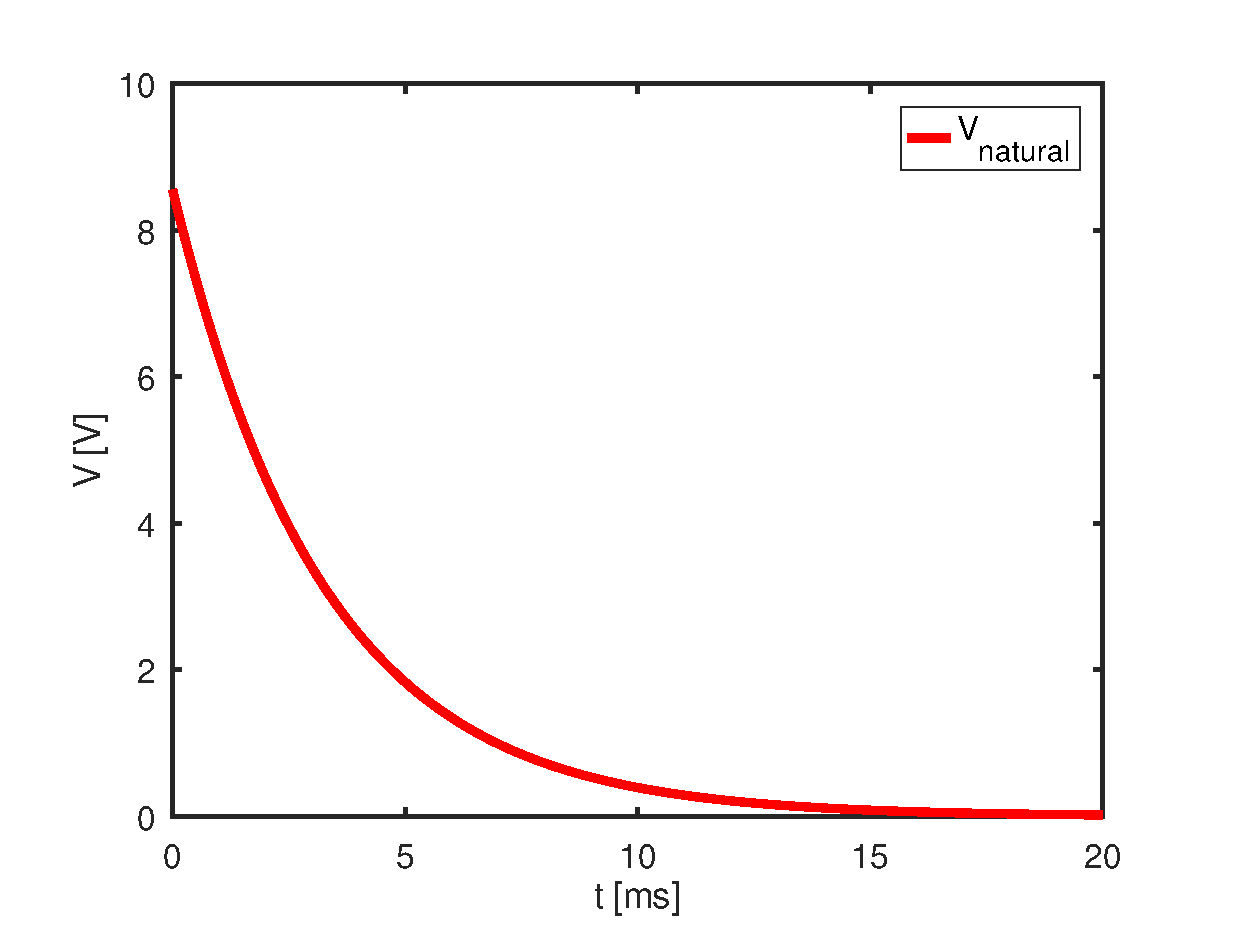
\includegraphics[width=0.5\linewidth]{natural.eps}
\caption{Circuit analysed.}
\label{fig:sim3}
\end{figure}


\subsection{Simulation Analysis}
In this section, a transient analysis was made in order to evaluate the natural response of the circuit, which means, the variation over time. The description of the circuit included the initial values of v(6) and v(8), calculated in question 1. As the ngspice and octave results matched, as observed in \ref{subsection:2.3}, the theorectical values were imported from a .cir file created by octave.
The time interval considered was [0,20]ms.
\begin{figure}[h] \centering
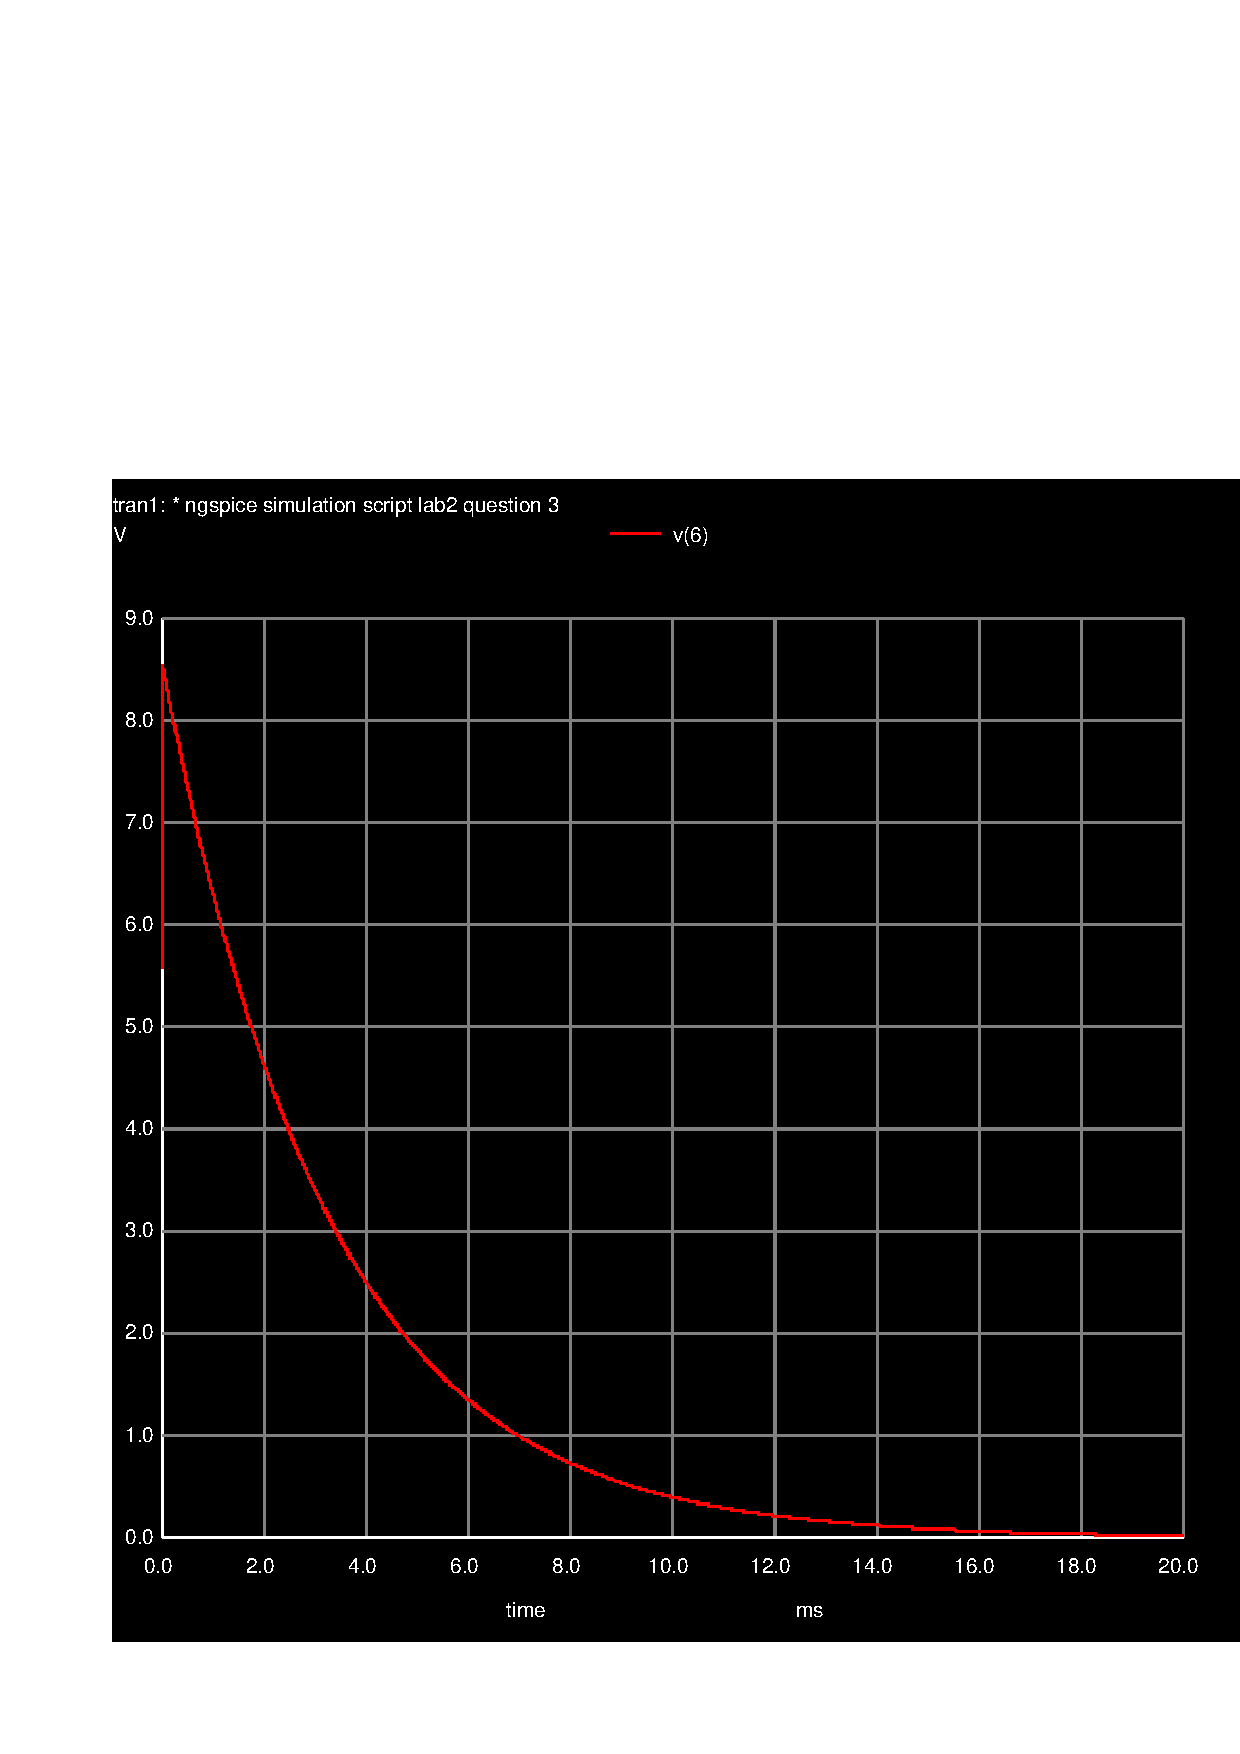
\includegraphics[width=0.5\linewidth]{sim3.pdf}
\caption{Circuit analysed.}
\label{fig:sim3}
\end{figure}
\newpage
